%\documentclass[letterpaper, 10 pt, conference]{ieeeconf}`
%\usepackage{filecontents,lipsum}
%\usepackage[noadjust]{cite}
%%\begin{filecontents*}{references.bib}
%%@article{Khoe:1994:CML:2288694.2294265,
%%    author = {Khoe, G. -D.},
%%    title = {Coherent multicarrier lightwave technology for flexible capacity networks},
%%    journal = {Comm. Mag.},
%%    issue_date = {March 1994},
%%    volume = {32},
%%    number = {3},
%%    month = mar,
%%    year = {1994},
%%    issn = {0163-6804},
%%    pages = {22--33},
%%    numpages = {12},
%%    url = {http://dx.doi.org/10.1109/35.267438},
%%    doi = {10.1109/35.267438},
%%    acmid = {2294265},
%%    publisher = {IEEE Press},
%%    address = {Piscataway, NJ, USA},
%%}
%%\end{filecontents*}
%\title{This document}
%\author{This author}

%%%%%%%%%%%%%%%%%%%%%%%%%%%%%%%%%%%%%%%%%%%%%%%%%%%%%%%%%%%%%%%%%%%%%%%%%%%%%%%%
%2345678901234567890123456789012345678901234567890123456789012345678901234567890
%        1         2         3         4         5         6         7         8

\documentclass[letterpaper, 10 pt, conference]{ieeeconf}  % Comment this line out if you need a4paper

%\documentclass[a4paper, 10pt, conference]{ieeeconf}      % Use this line for a4 paper

\IEEEoverridecommandlockouts                              % This command is only needed if 
                                                          % you want to use the \thanks command

\overrideIEEEmargins                                      % Needed to meet printer requirements.

% See the \addtolength command later in the file to balance the column lengths
% on the last page of the document

% The following packages can be found on http:\\www.ctan.org
%\usepackage{graphics} % for pdf, bitmapped graphics files
%\usepackage{epsfig} % for postscript graphics files
%\usepackage{mathptmx} % assumes new font selection scheme installed
%\usepackage{times} % assumes new font selection scheme installed
%\usepackage{amsmath} % assumes amsmath package installed
%\usepackage{amssymb}  % assumes amsmath package installed
%\usepackage{filecontents,lipsum}
%\usepackage[noadjust]{cite}
%\usepackage{bm}
%\usepackage{tikz}
%\usepackage{graphicx}
%\usepackage{caption}
%\usepackage{subcaption}
%\usepackage{multicol}
%\usepackage{url}
%\usepackage{geometry}
%\usepackage{mathtools}
%\usepackage[utf8]{inputenc}
%\usepackage[english]{babel}
%\usepackage{algorithm}
%\usepackage[]{algpseudocode}


\usepackage{afterpage}
\usepackage{algorithm}
\usepackage[]{algpseudocode}

\usepackage{stix}
\usepackage{amssymb}
\usepackage{amsmath}

%\DeclareMathAlphabet\mathcal{OMS}{cmsy}{b}{n}
%\usepackage[math-style=TeX, bold-style=TeX]{unicode-math}

\usepackage{arydshln}
\usepackage[english]{babel}
\usepackage{bm}
\usepackage{caption}
\usepackage[T1]{fontenc}
\usepackage[]{graphicx}
\graphicspath{ {./fig/} }

\usepackage[utf8]{inputenc}
\usepackage{marginnote}
\usepackage{multicol}
\usepackage[T1]{xcolor}
\usepackage{soul}
\usepackage{subfig}
\usepackage{tikz}
\usepackage{url}
\usepackage[backend=biber,style=ieee,sorting=none]{biblatex}
\addbibresource{bib/references.bib}


\newcommand{\trsp}{{^{\top}}}

\newcommand\blankpage{%
    \null
    \thispagestyle{empty}%
    \addtocounter{page}{-1}%
    \newpage}

\newcommand*\circled[1]{\tikz[baseline=(char.base)]{
            \node[shape=circle,draw,inner sep=2pt] (char) {#1};}}

\newcommand*{\important}[1]{\textcolor{red}{\danger~\textbf{IMPORTANT:~}} \textcolor{red}{#1}}

\newcommand*{\pending}[1]{\textcolor{blue}{$\bigstar$~\textbf{PENDING~#1}}}

\newcommand\mybox[2][]{\tikz[overlay]\node[fill=blue!100,inner sep=4pt, anchor=text, rectangle, rounded corners=1mm,#1] {#2};\phantom{#2}}

\newcommand{\TODO}{\mybox[fill=yellow]{\textcolor{blue}{\Large \textbf{TODO}}}}
\newcommand\myhl[1]{\textcolor{red}{#1}}


\newtheorem{prop}{Proposition}

\usepackage[nolist]{acronym}
\newacro{smc}[SMC]{sensorimotor contingencies}
\newacro{dfc}[DFC]{dynamic functional connectivity}
\newacro{fc}[FC]{functional connectivity}
\newacro{nnmf}[NNMF]{non-negative matrix factorization}
\newacro{imi}[IMI]{instantaneous mutual information}
\newacro{irm}[IRM]{infinite realtional model}
\newacro{mi}[MI]{mutual information}

\newacro{}[]{}
\newacro{}[]{}
\newacro{}[]{}

\title{\LARGE \bf
An analytical framework for the discovery of body features and behaviors from sensorimotor dynamic functional connectivity
}


\author{Fernando D\'iaz Ledezma, Valentin Marcel, and Matej Hoffmann}

\begin{document}
\maketitle
% ---
\begin{figure*}[h!]
	\centering
	\includegraphics[width=0.95\textwidth]{sensorimotor_dfc_framework.png}
	\caption{\textbf{Analysis of the sensorimotor \acl{dfc}.} Motion excites the sensorimotor system of a robotic agent. While moving, the sensorimotor functional connectivity changes over time.}
	\label{fig:general_overview}
\end{figure*}
% ---
\begin{abstract}
\myhl{Regularities present in the somatosensory signals of a robotic agent can reflect its embodiment and the associations resulting from an active control policy. In this work, we analyze the dynamic functional connectivity of the somatosensory signals based on the instantaneous pairwise mutual information. As the robot performs exploratory motions based on motor babbling, we capture and study the time-varying changes in the signal relationships. We analyze the instantaneous and average information sharing and associate them with different information states. A simulated planar system study shows that using instantaneous mutual information to extract and leverage the relationships between the agent's somatosensory signals exhibited during exploratory motions can yield information related to self-touch events.}\pending{Needs to be re-worked}
\end{abstract}
% =============================================================================
%                                                                             |
%                                                                             |
% ------------------------------- SECTION ------------------------------------|
%                                                                             |
%                                                                             |
% =============================================================================
\section{Introduction}\label{sec:intro}
Understanding the brain’s structural and \ac{fc} has significantly advanced our knowledge of its organization and information-processing capabilities. A similar approach can be applied to studying the sensorimotor signals of an embodied agent, offering insights into how the agent processes information and adapts its behavior. While analyzing the structural connectivity of these signals may not always be feasible, investigating their functional connectivity provides a powerful way to understand an agent’s body structure and the emergence of behavior through information acquisition. A key concept in this context is that of \ac{smc} \cite{Jacquey2019Sensorimotorcontingenciesas}, the regularities and dependencies between an organism's actions (motor actions) and the resulting sensory feedback linking an agent’s sensorimotor signals to its physical embodiment and the world. Identifying and analyzing these regularities using information-theoretic methods can help uncover fundamental principles of sensorimotor learning. 


% SUBSECTION ==================================================================
\subsection{Related works}
Research suggests that \acp{smc} play a fundamental role in acquiring body knowledge, generalization, and goal-directed behavior \cite{Jacquey2019Sensorimotorcontingenciesas}. As such, they can be viewed as a form of sensorimotor representation---a framework that enables an embodied agent to learn, adapt, and interact with its environment. Despite extensive research on sensorimotor representations \cite{Nguyen2021Sensorimotorrepresentationlearning}, the precise relationship between sensorimotor regularities, body knowledge, and behavior remains an open question.

Several studies have used information-theoretic metrics to examine these relationships in sensorimotor systems \cite{Schmidt2013Bootstrappingperceptionusing,Lungarella2006Mappinginformationflow,Polani2009Modelsinformationprocessing,Bossomaier2016introductiontransferentropy,Olsson2006unknownsensorsactuators}. Among different sensory modalities, touch has been identified as particularly crucial in understanding \acp{smc}. For example, Gama et al. \cite{Gama2021Goaldirectedtactile} demonstrated how intrinsic motivation and goal-babbling can facilitate self-touch learning in a simulated humanoid robot with artificial tactile skin. Similarly, Roncone et al. \cite{Roncone2014Automatickinematicchain} showed that self-touch could be used for kinematic calibration, allowing a robot to close its kinematic chain autonomously by touching its own body. Marcel et al. \cite{Marcel2022Learningreachown} further explored self-touch representation using a denoising framework with a multimodal variational autoencoder, enabling a robot to reconstruct its self-reaching configurations internally.

Another relevant area of study is \ac{dfc}, which explores how the statistical properties of sensorimotor signals evolve over time. Originally applied in neuroscience, \ac{dfc} has been used to detect states of reduced functional connectivity during epilepsy onsets \cite{Christiaen2020Dynamicfunctionalconnectivity} and to identify abnormal connectivity patterns in brains affected by illness \cite{Zhou2020Earlychildhooddevelopmental}. More recently, \ac{dfc} has been used to investigate how sensorimotor connectivity evolves in simulated infants as they develop \cite{Kanazawa2023Openendedmovements}.

In robotics, functional connectivity is expected to change based on the robot’s motion policy or the task it performs. Capturing and analyzing these evolving patterns using \ac{dfc} could provide a deeper understanding of how an agent’s sensory and motor systems interact over time.

% SUBSECTION ==================================================================
\subsection{Overview}
This work introduces an analytical framework, illustrated in Fig.~\ref{fig:general_overview}, to investigate the formation of relationships between the sensorimotor signals of a simulated two-dimensional embodied agent. Specifically, the framework examines the time-varying \acl{fc} between the agent's proprioceptive, tactile, and visual inputs. During an initial exploratory phase using motor babbling, the agent gathers information about its evolving sensorimotor relationships. The framework models these changing relationships as time-varying graphs, serving as a proxy for understanding the formation and evolution of \acp{smc}. To achieve this, we compute the instantaneous pairwise \ac{mi}, capturing the \acl{dfc} that correlates the agent’s information-sharing state with its motion and potential interactions. A key step in the framework involves applying a Bayesian approach to uncover hidden structures within the mutual information-based connectivity. This analysis identifies clusters of highly related signals and their evolving interactions over time. Finally, the framework decomposes these dynamic relationships to extract meaningful patterns (i.e., subgraphs) in the graphs, which represent distinct information-sharing states. The insights derived from these states and their transitions reveal fundamental aspects of the agent’s body structure and behavior.
% ---
\begin{figure}[!t]
	\begin{center}
		\hspace*{\fill}
		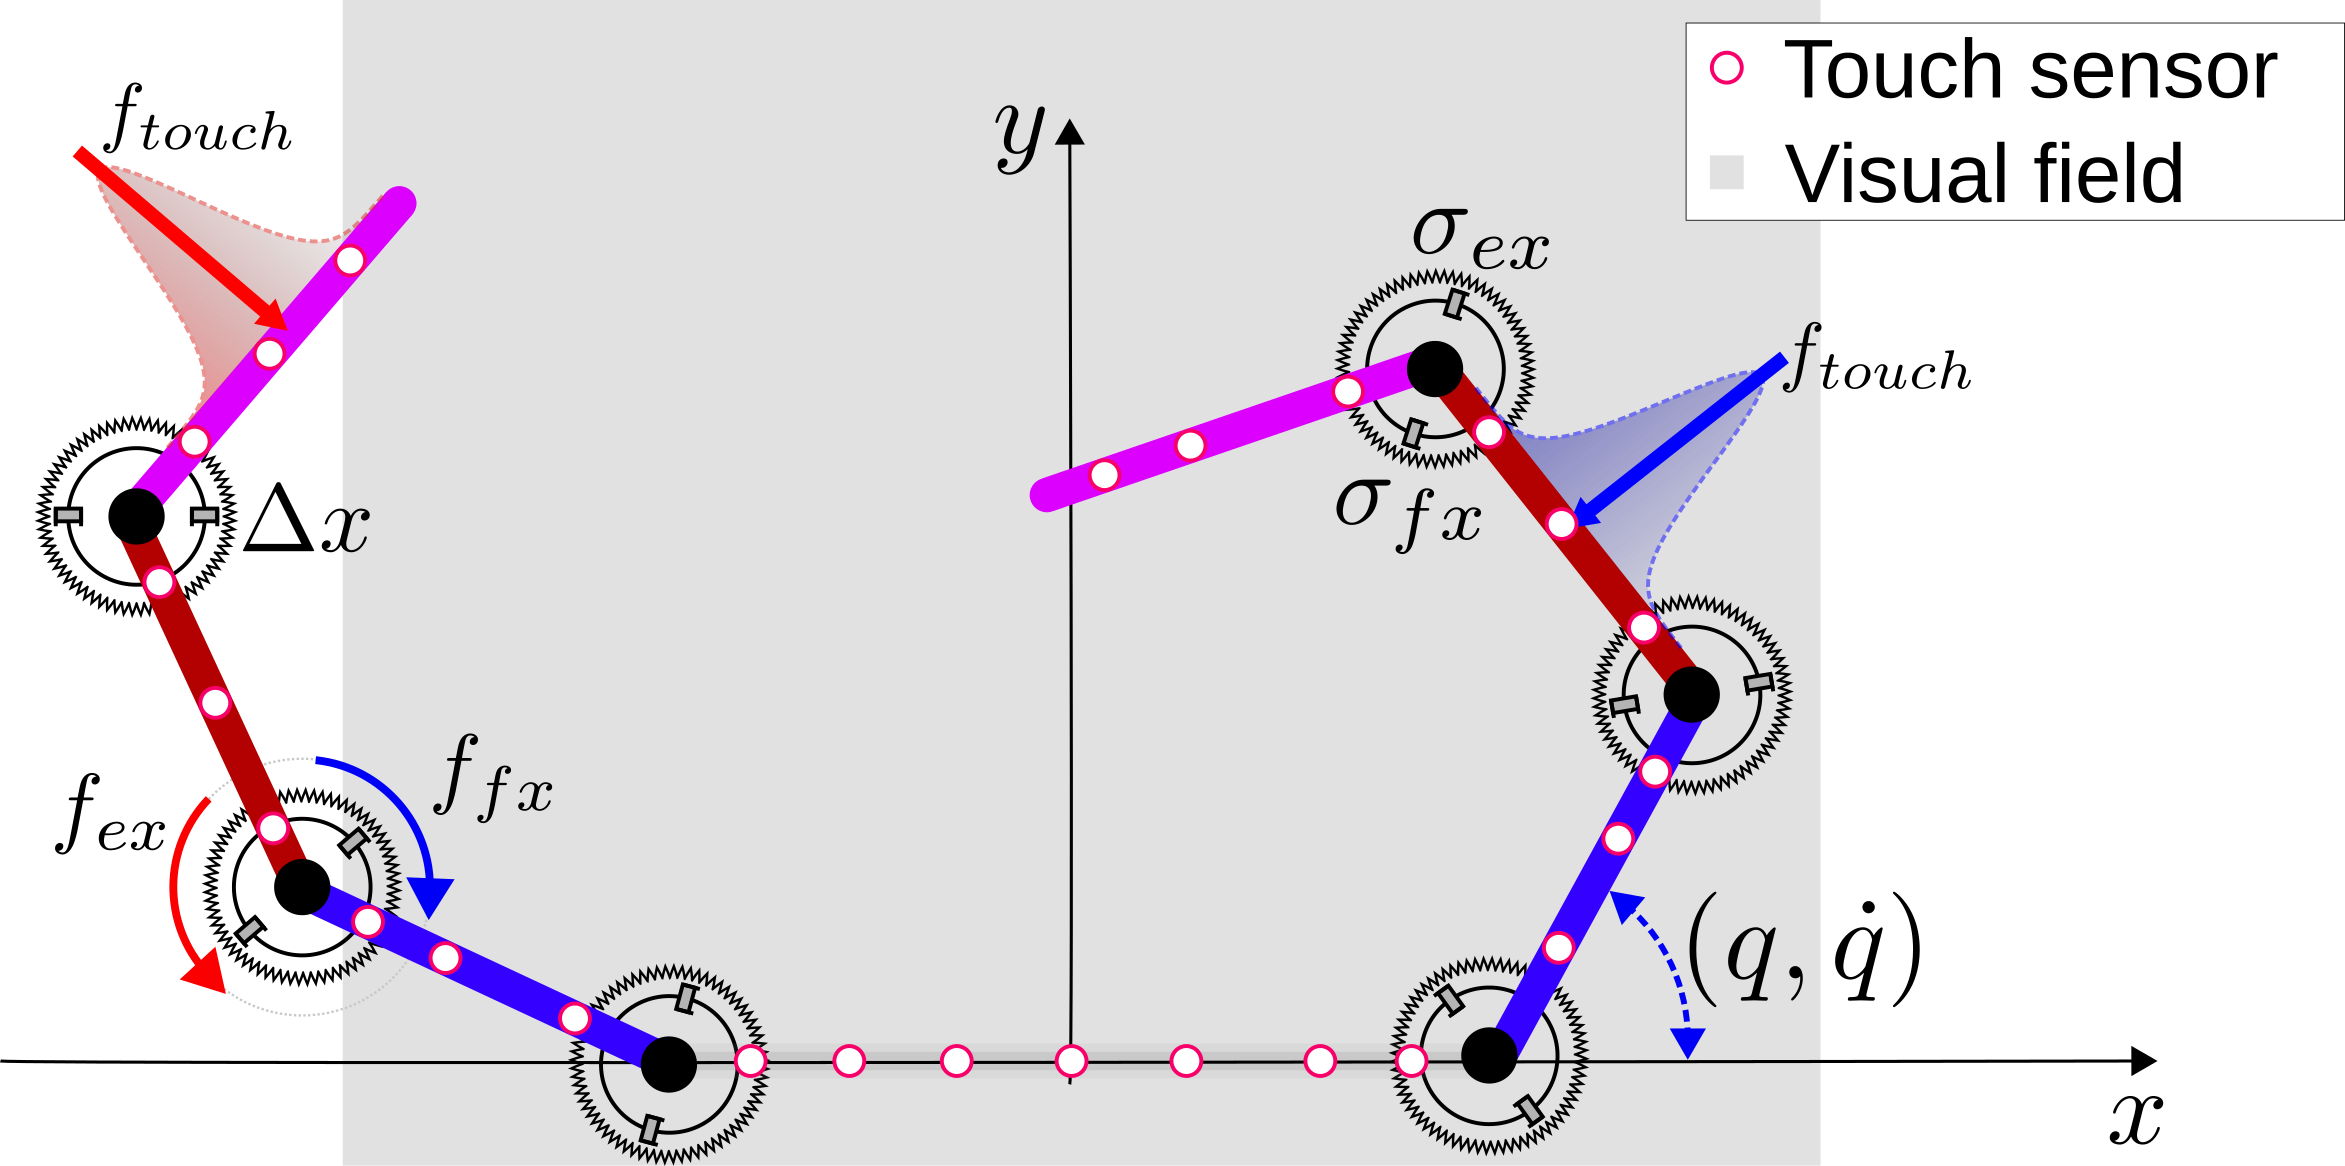
\includegraphics[width=0.99\columnwidth]{extended_planar_dual_arm_with_vision.png}
		\hspace*{\fill}
	\end{center}
	\caption{\label{fig:extended_dual_arm_robot} \textbf{The embodied agent.} The planar dual arm robot with antagonistic actuation, tactile modules and vision.}
\end{figure}
% ---

% =============================================================================
%                                                                             |
%                                                                             |
% ------------------------------- SECTION ------------------------------------|
%                                                                             |
%                                                                             |
% =============================================================================
\section{The embodied agent}\label{sec:the_embidied_agent}
% SUBSECTION ==================================================================
\subsection{The planar dual arm model}
We employ the robot model described in \cite{Mannella2018Knowyourbody,Marcel2022Learningreachown} as our reference system. This model consists of a simple planar dual-arm system with six degrees of freedom, featuring three links per arm and a fixed torso, see Fig.~\ref{fig:extended_dual_arm_robot}. The robot is equipped with tactile sensors distributed across its body. To instantiate the dynamics of the model, inertial properties are assigned to the robot's composing bodies. Its actuation mechanism is based on a biologically-inspired model presented in \cite{Ekeberg1993combinedneuronalmechanical,Wadden1998neuromechanicalmodel, Shim2012Chaoticexplorationlearning}, where the position $q$ and velocity $\dot{q}$ of each joint is driven by antagonistic muscles (modeled as spring-damper systems). The pulling force these muscles exert is linearly controlled by the signal generated by a corresponding motor neuron $\sigma$. The joint torque,
% ---
\begin{equation}\label{eq:antagonistic_torque}
	\tau = \alpha \left(\sigma_\mathrm{fx} - \sigma_\mathrm{ex}\right)  + \beta \left(\sigma_\mathrm{fx} + \sigma_\mathrm{ex} + \gamma \right) q + \delta \dot{q},
\end{equation}
% ---
results from the difference between activation signals for flexion $ \sigma_\mathrm{fx} $ and extension $\sigma_\mathrm{ex}$. These activation signals contribute to the flexion and extension pulling forces, $ f_\mathrm{fx}$ and $f_\mathrm{ex} $, respectively. The remaining parameters in the model account for the muscle force gain ($\alpha$), stiffness gain ($\beta$), tonic stiffness ($\gamma$), and damping coefficient ($\delta$).

% SUBSECTION ==================================================================
\subsection{The sensory signals}
%Randomly located tactile sensors along the robot's one-dimensional body are modeled based on population coding \cite{Panzeri2010PopulationCoding}. They are represented as distance-dependent Gaussian receptive fields---see Fig.~\ref{fig:population_coding}---whose mean is dictated by the tactile sensor location. 
%To incorporate touch strength into the model, we adjust the distance-based activation of the Gaussian receptive fields based on the contact force. Similarly, the proprioceptive measurements of the robot are also encoded using receptive fields. Ultimately, our extended model results in a vector $\bm{s}$ containing a number $N_s$ of somatosensory signals encompassing proprioception (joint position $\bm{p}$, velocity $\bm{v}$, and effort $\bm{e}$) and touch-strength-modulated tactile signals $\bm{r}$; i.e.:
%% ---
%\begin{equation}
%	\bm{s} = \begin{bmatrix}
%		\bm{p}\trsp & \bm{v}\trsp & \bm{e}\trsp & \bm{r}\trsp
%	\end{bmatrix}\trsp \in \mathbb{R}^{N_s}_{\geq}.
%\end{equation}
%%---
%\myhl{In addition to somatosensation, we equip the robot with visual inputs. The visual sensors are composed of a fixed, rectangular, pixel grid of size $(s_\text{x},s_\text{y})$ with  $(n_\text{x},n_\text{y})$ pixels in each direction. Pixels are sensitive to the positions of the agent's limbs; e.g., when a limb segment intersects with the rectangular pixel receptive field in the 2D space, its value is updated to one. To simulate some visual sensors' spatial overlap~\cite{Marshall2015}, we perform a convolution of the pixel values image with a 3-by-3 kernel mapping to get the visual sensors' activations.}

%Randomly located tactile sensors along the robot's one-dimensional body are modeled based on population coding \cite{Panzeri2010PopulationCoding}. They are represented as distance-dependent Gaussian receptive fields---see Fig.~\ref{fig:population_coding}---whose mean is dictated by the tactile sensor location. To incorporate touch strength into the model, we adjust the distance-based activation of the Gaussian receptive fields based on the contact force. Similarly, the proprioceptive measurements of the robot are also encoded using receptive fields. In addition to somatosensation, we equip the robot with visual inputs. The visual sensors are composed of a fixed pixel receptive field with $(n_\text{x},n_\text{y})$ pixels in each direction. When a limb segment intersects with a pixel in the visual field, its value is updated to one; i.e., the pixels are sensitive to the positions of the agent's limbs. Additionally, to simulate spatial overlap in some of the visual sensors~\cite{Marshall2015}, we perform a convolution of the pixel values image with a 3-by-3 kernel mapping to get the pixel receptive field's activations.
%
%Ultimately, in our extended model, $N_s$ signals encompassing position-based proprioception, touch-strength-modulated tactile sensation $\bm{r}$, and visual inputs $\bm{v}$ form a vector
%% ---
%\begin{equation}
%	\bm{s} = \begin{bmatrix}
%		\bm{p}\trsp & \bm{r}\trsp & \bm{v}\trsp
%	\end{bmatrix}\trsp \in \mathbb{R}^{N_s}_{\geq}.
%\end{equation}
%%---
%of somatosensory signals. In stage \circled{1} of our proposed analytical framework, perceptual system of the embodied agent is excited to collect the signals $\bm{s}$ following a motor babbling strategy. 


Tactile sensors are randomly distributed along the robot's one-dimensional body and modeled using population coding \cite{Panzeri2010PopulationCoding}. Each sensor is represented by a Gaussian receptive field, whose mean is determined by the sensor's location. %n—see Fig.~\ref{fig:population_coding}. 
To incorporate touch strength, we modulate the activation of each receptive field based on the contact force, adjusting the distance-dependent response accordingly.  

Similarly, the robot's proprioceptive measurements are also encoded using Gaussian receptive fields. In addition to somatosensation, the robot is equipped with visual inputs. The visual sensors consist of a fixed pixel receptive field with dimensions $(n_\text{x}, n_\text{y})$. When a limb segment intersects with a pixel in the visual field, the pixel value is set to one---i.e., pixels are sensitive to the positions of the agent's limbs. To account for spatial overlap in some visual sensors~\cite{Marshall2015}, we apply a convolution operation using a 3-by-3 kernel, to obtain the final pixel receptive field activations.  

Ultimately, in our extended model, the visuo-somatosensory signal vector consists of $N_\text{s}$ signals, including position-based proprioception ($\bm{p}$), touch-strength-modulated tactile sensation ($\bm{r}$), and visual inputs ($\bm{v}$):  
% ---
\begin{equation}
	\bm{s} = \begin{bmatrix}
		\bm{p}\trsp & \bm{r}\trsp & \bm{v}\trsp
	\end{bmatrix}\trsp \in \mathbb{R}^{N_\text{s}}_{\geq}.
\end{equation}
%---
In stage \circled{1} of our proposed analytical framework, the perceptual system of the embodied agent is stimulated to collect the signals $\bm{s}$ through a motor babbling strategy.

%% ---
%\begin{figure}[!t]
%	\begin{center}
%		\hspace*{\fill}
%		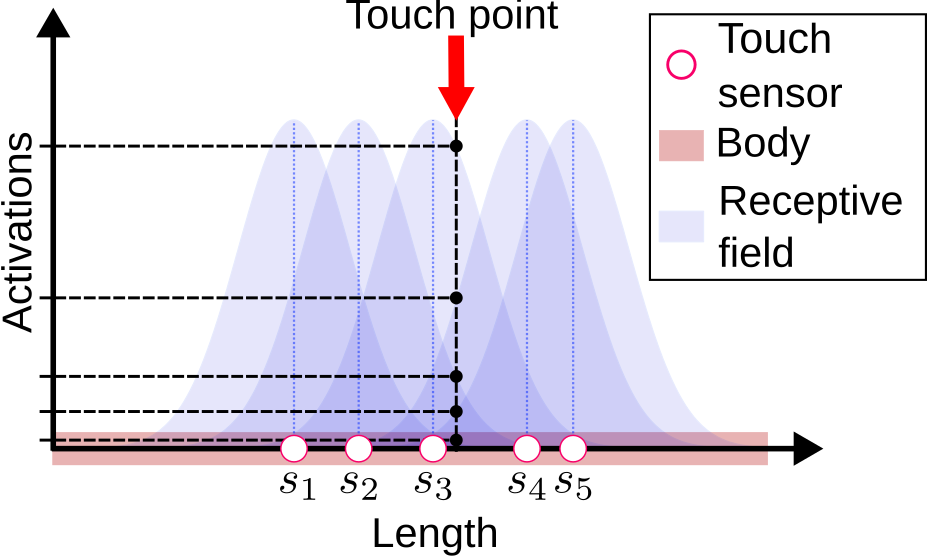
\includegraphics[width=0.75\columnwidth]{touch_receptive_fields.png}
%		\hspace*{\fill}
%	\end{center}
%	\caption{\label{fig:population_coding} \textbf{Population coding.} The receptive fields encode a signal into several distance-based activation functions.}
%\end{figure}
%% ---
% =============================================================================
%                                                                             |
%                                                                             |
% ------------------------------- SECTION ------------------------------------|
%                                                                             |
%                                                                             |
% =============================================================================
\section{The sensorimotor dynamic functional connectivity}

% Subsection ==================================================================
\subsection{\Acl{fc}}
% \ac{fc} is a method for network topology inference that characterizes the dependencies of the observed signals from a system based on their probability distributions \cite{Friston2011Functionaleffectiveconnectivity}. It can be subdivided into undirected and directed, the latter being related to the analysis of statistical causation from the data \cite{Bastos2016tutorialreviewfunctional}. By studying the \ac{fc}, it is possible to reveal a structure that aids in analyzing the interaction among the entities in a network.
% \ac{fc} is a method for network topology inference that characterizes the dependencies of the observed signals from a system based on their probability distributions \cite{Friston2011Functionaleffectiveconnectivity}. By studying the \ac{fc}, it is possible to reveal a structure that aids in analyzing the interaction among the entities in a network.

% Based on the connection between embodiment and information structure \cite{Pfeifer2007Selforganizationembodiment}, we hypothesize that bodily structural properties and motor behaviors of an embodied agent can be made apparent by studying the \ac{fc} among the sensorimotor signals $ \bm{s}(t) $. From the various metrics that have been proposed to evaluate such relationships, we, in particular, leverage those based on information theory \cite{Bonsignorio2020EntropyBasedMetrics,Bonsignorio2013Quantifyingevolutionaryself}, as their model-free nature can capture linear and nonlinear relationships between signals. Particularly, we use \ac{mi}, a quantity that has been applied in different contexts to quantify the relationships between variables \cite{Steuer2002mutualinformationdetecting}. 

\ac{fc} is a method for inferring network topology by characterizing the dependencies between observed signals based on their probability distributions \cite{Friston2011Functionaleffectiveconnectivity}. Analyzing \ac{fc} helps uncover underlying structures describing interactions between network entities. Building on the connection between embodiment and information structure \cite{Pfeifer2007Selforganizationembodiment}, we hypothesize that an embodied agent’s bodily structural properties and motor behaviors can be revealed by studying the \ac{fc} among its sensorimotor signals $\bm{s}(t)$. To quantify these relationships, we leverage information-theoretic measures \cite{Bonsignorio2020EntropyBasedMetrics,Bonsignorio2013Quantifyingevolutionaryself}, as their model-free nature captures both linear and nonlinear dependencies between signals. In particular, we focus on \ac{mi}, a widely used measure for quantifying relationships between variables across different domains \cite{Steuer2002mutualinformationdetecting}.

Given the Shannon's entropy of a variable $X$  
% ---
\begin{equation}\label{eq:entropy}
	H(X) = -\sum_{i=1}^{n}p(x_i)\text{log}_2\left(p\left(x_i\right)\right)
\end{equation}
% ---
and the joint entropy between two variables $ X $ and $ Y $ 
% ---
\begin{equation}\label{eq:joint_entropy}
	H(X,Y) = -\sum_{i=1}^{n}\sum_{j=1}^{n} p(x_i,y_j)\text{log}_2\big(p\left(x_i,y_j\right)\big),
\end{equation}
% ---
the \ac{mi} between two signals 
% ---
\begin{equation}\label{eq:mutual_information}
	I\left(X;Y\right) =I\left(Y;X\right) = H(X) + H(Y) - H(X,Y)
\end{equation}
% ---
can be interpreted as the amount by which a random signal $ Y $ reduces the uncertainty about a random signal $ X $ \cite{Cover1999Elementsinformationtheory}. It is a symmetric measure of the information sharing by both signals that depends on their marginal $p(\cdot)$ and joint $p(\cdot,\cdot)$ probability distributions.

By extension, the \ac{mi} matrix $\bm{\mathcal{I}} \in \mathbb{R}^{{N_\text{s}} \times {N_\text{s}}}$ can be constructed by computing the pairwise \ac{mi} between the $\left\lbrace s_i\right\rbrace^{N_\text{s}}_{i=1}$ sensorimotor signals. In practice, computing an entry
% ---
\begin{equation}\label{eq:adjacency_mi}
	\left(\bm{\mathcal{I}}\right)_{i,j} = I(s_i;s_j)
\end{equation}
% ---
for a pair $\left({s}_i(t),{s}_j(t)\right)$ involves centering their samples---to zero mean and unit standard deviation---and using either binning, kernel, or nearest neighbor methods to compute their \ac{mi} \cite{WaltersWilliams2009Estimationmutualinformation}. In this work, we used a binning strategy to compute $\bm{\mathcal{I}}$. 

% ---
\begin{figure}[!t]
	\begin{center}
		\hspace*{\fill}
		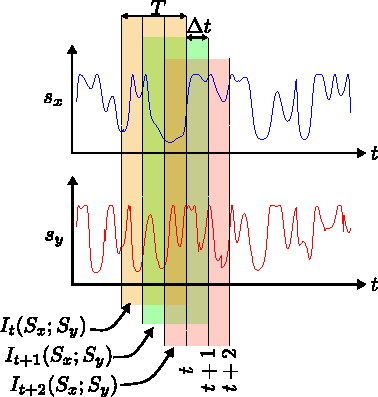
\includegraphics[width=0.7\columnwidth]{sliding_window_mi.pdf}
		\hspace*{\fill}
	\end{center}
	\caption{\label{fig:mi_sliding_window_mi} \textbf{\Acl{imi}.} A sliding window strategy is used to compute the \ac{mi} in an interval $\left[t-T,t\right]$.}
\end{figure}
% ---
% Subsection ==================================================================
\subsection{\Acl{dfc}}
When analyzing \ac{fc}, it might be interesting to look not only at the aggregated effect of a complete dataset of recordings but also at the instantaneous changes that occur in the relationships. Indeed, the functional relationships between sensorimotor signals can change rapidly depending on the motion policy and the agent's interaction with the environment. To capture this time-varying, i.e., dynamic, \acl{fc}, it is common to use a sliding time window \cite{Preti2017dynamicfunctionalconnectome} with forward step $\Delta t$ from which the \ac{mi} is computed only for a small number of samples.

For a time window of length $T$, the \ac{mi} $I_t(s_x(t);s_y(t))$ between a distinct pair of signals $s_x(t)$ and $s_y(t)$ at time $t$ is computed using the set of signal samples spanning the $\left[t-T,t\right]$ interval, as illustrated in Fig.~\ref{fig:mi_sliding_window_mi}. We refer to this quantity as the \acf{imi}. 

By extension, in stage $\circled{2}$ in Fig.~\ref{fig:general_overview}, the \ac{mi} matrix $\bm{\mathcal{I}}(t)$ at time $t$ is constructed by calculating the \ac{imi} for all pairwise signals within the same time interval. The temporal evolution of this time-varying \ac{mi} matrix $\bm{\mathcal{I}}(t)$ captures the \ac{dfc} between the sensorimotor signals.

% Subsection ==================================================================
\subsection{Finding structure in the functional relationships}\label{sec:the_irm}
Analyzing the time-varying relationships in $\bm{\mathcal{I}}(t)$ at a local level may not be as informative as examining the global structure defined by interactions between groups of signals. To address this, we first identify clusters of closely related signals based on their \ac{mi} values. However, conventional clustering techniques typically require a predetermined number of clusters. To overcome this limitation, in stage \circled{3} of our framework, we employ a Bayesian approach---the \ac{irm}~\cite{Moerup2012}---to uncover hidden structures within the \ac{mi}-based connectivity.

This probabilistic framework groups entities (e.g., signals) into $N_\text{c}$ clusters, while simultaneously learning the relationships between them. Its primary objective is to group entities into clusters based on their relationships and predict new relationships based on these assignments. The \ac{irm} utilizes a Chinese Restaurant Process or a Dirichlet Process, allowing the number of clusters to dynamically expand as needed. By leveraging probabilistic methods, the \ac{irm} estimates the likelihood of entities belonging to the same cluster and models inter-cluster relationships using probability distributions.

For our purposes, the \ac{irm} taskes as an input the time series of  \ac{imi}-matrices---representing $N$ samples $\left\lbrace \bm{\mathcal{I}}(k)\right\rbrace^{N}_{k=1}$---and assigns to the i-th signal in $\bm{s}$ a cluster $z_i$. To identify these latent cluster relationships, \ac{irm} assumes that the probability of a relation between two entities depends only on their cluster memberships. Specifically, if two entities belong to clusters $z_i$ and $z_j$, the probability of a connection is determined by a parameter $\theta_{z_i,z_j}$. These inter-cluster probabilities form a new bynary relational matrix $\bm{Z}\in \mathbb{R}^{N_\text{c}\times N_\text{s}}$, which the model infers from data. Additionally, the \ac{irm} produces a matrix $\bm{H}\in \mathbb{R}^{N_\text{c}\times N_\text{c} \times N}_{\geq}$, which captures the probability of relations between clusters.

% Subsection ==================================================================
\subsection{Analyzing recurring patterns}
The matrices $(\bm{Z}, \bm{H})$ in Sec.~\ref{sec:the_irm} capture the global changing relationships between the sensorimotor signals. In stage $\circled{4}$, the goal is to utilze the $N$ relationships captured in $\bm{H}$ to identify recurrent patterns in the \ac{fc} that corresnpond to distinct motor behaviors of the agent. Additionally, assessing the strenght and frequency of these patterns is crucial to determine their significance. 

Common approaches to detect repeating patterns in \ac{dfc} include the cosine similarity~\cite{Menon2019comparisonstaticdynamic}, k-means clustering~\cite{Li2017Hightransitionfrequencies}, and  \ac{nnmf}~\cite{Fu2019Nonnegativematrixfactorization}. We selected the latter, due to its demonstrated  effectiveness in analyzing brain dynamic functional networks and its application in community  detection~\cite{Wang2011Communitydiscoveryusing,Luo2021Symmetricnonnegativematrix}.

To use \ac{nnmf}, a matrix $\bar{\bm{H}}\in \mathbb{R}^{N_\text{r}\times N}$ is constructed by vectorizing  and concatenating each of the matrices in $\bar{\bm{H}}$; where $N_\text{r} = N_\text{c}(N_\text{c}-1)/2$ is the total number of pairwise relationships. Since this matrix is strictly non-negative, it is amenable to be decomposed and analyzed using \ac{nnmf}. Then, the \ac{nnmf} algorithm can be used to split the nonnegative matrix $\bar{\bm{H}}$ into two parts: a matrix $\bm{F} \in \mathbb{R}^{N_\text{f}\times N_\text{r}}_{\geq}$ of $N_\text{f}$ basis (or factors) and a matrix $\bm{W} \in \mathbb{R}^{N\times N_\text{f}}_{\geq}$ of their corresponding contributions such that
% ---
\begin{equation}
	\bar{\bm{H}}^\intercal \approx \bm{W} \bm{F}.
\end{equation}
% ---
%\begin{figure}[!t]
%	\centering
%	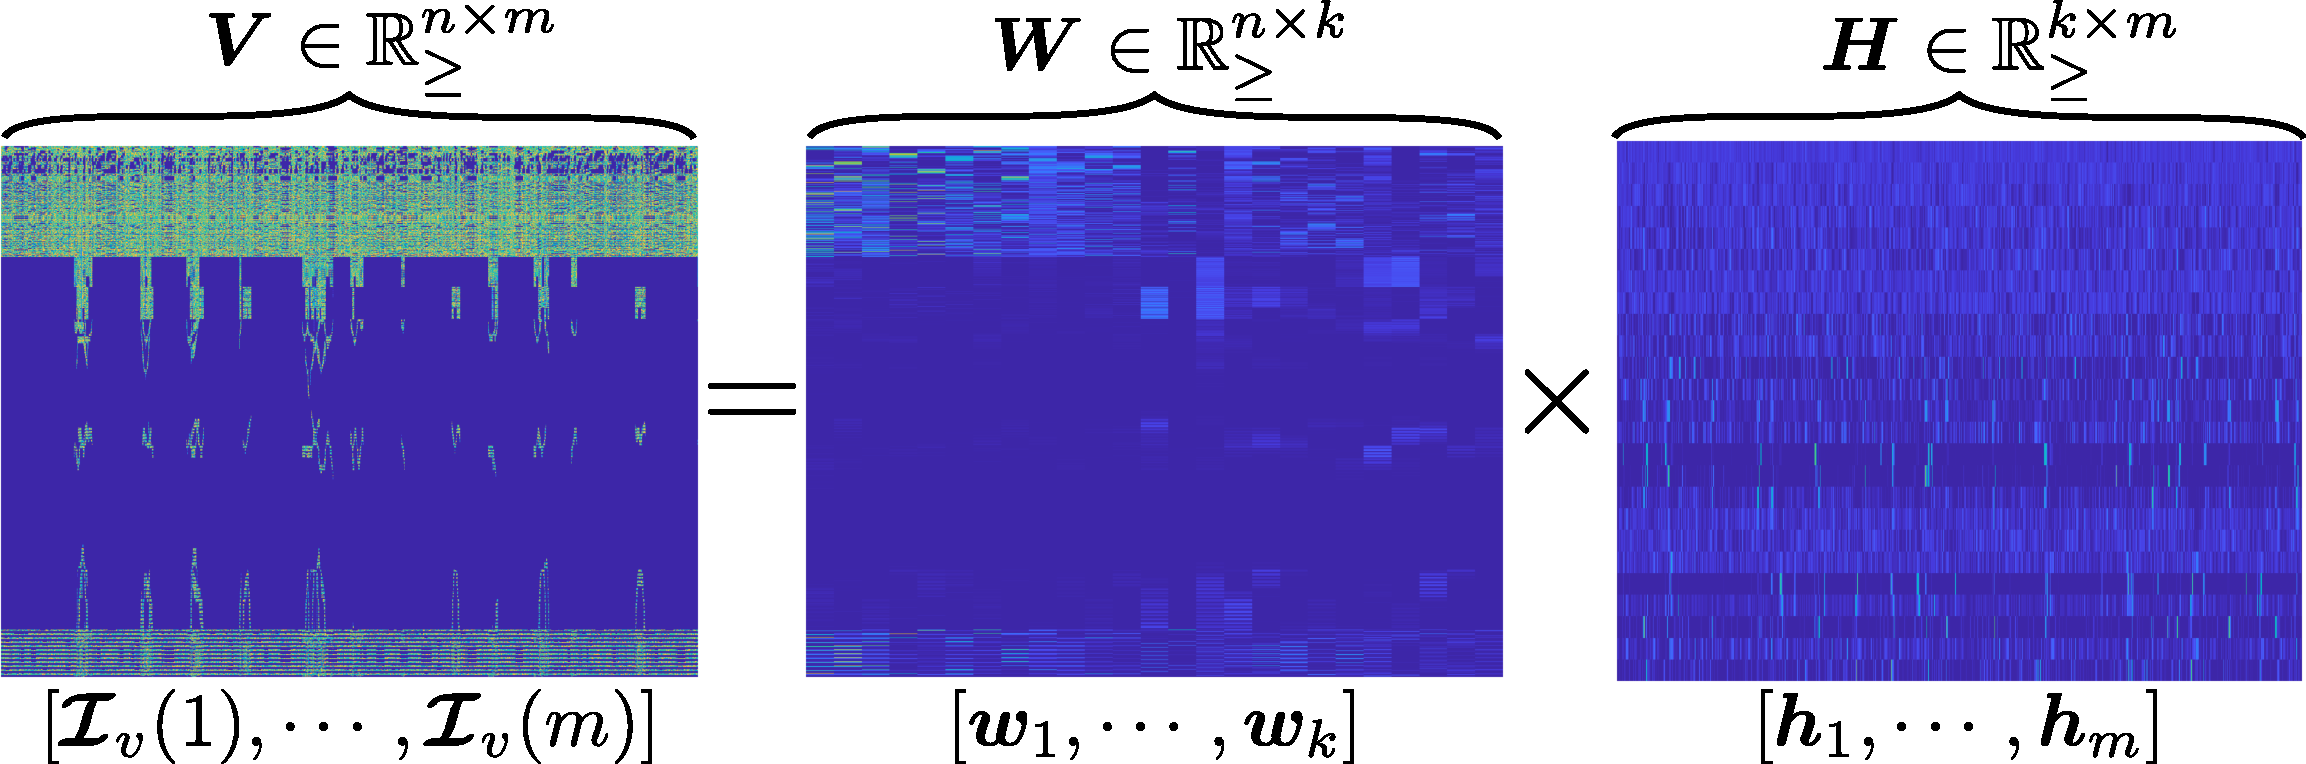
\includegraphics[width=0.99\columnwidth]{fig/nnmf_concept.pdf}
%	\caption{\textbf{Non-negative matrix factorization.} Decomposition of the \ac{imi} data matrix $\bm{S}$ using \ac{nnmf} helps identifying recurring patterns.\pending{Replace the matrices with actual data}}
%	\label{fig:nnmf}
%\end{figure}
% ---
To reiterate, \ac{nnmf} decomposes the sensorimotor \ac{dfc} captured in $\bm{H}$ into two key components: (1) a set of overlapping patterns $\bm{F}$---i.e., subnetworks---that evolve across space and time and (2) corresponding coefficient time series $\bm{W}$ that indicate the contribution of each subnetwork at a given time.

\myhl{One crucial question is the number of factors $k$ used to approximate the original dataset. From the various methods to select an adequate number \cite{Muzzarelli2019RankSelectionNon}, we chose $k$ following the elbow method as in \cite{Phalen2020Nonnegativematrix} by performing \ac{nnmf} for ascending values of $k$ and selecting the value where the residual error is not reduced any further.}

% Subsection ==================================================================
\subsection{Factors and \acp{smc}}
Each of the $N_\text{f}$ factors in $\bm{F}$ can be interpreted as a basis \ac{fc} graph capturing a state of information sharing between the $N_\text{c}$ sensorimotor clusters. They also encode patterns of motor interaction of the agent with its body. Cricually, the patterns in $\bm{F}$ can also be understood as proxis that represent \acp{smc} that were idifentified during the motor babbling phase. Other observed interaction patterns of the agent at a given time instant can be thought as an aggregation of the \acp{smc} using the entries of the coefficient matrix $\bm{W}$.

% XXXXXXXXXXXXXXXXXXXXXXXXXXXXXXXXXXXXXXXXXXXXXXXXXXXXXXXXXXXXXXXXXXXXXXXXXXXXXX
%Intuitively, NMF decomposes functional brain networks into the following: (1) a set of subnetworks (patterns) overlapping in space and
%time and (2) corresponding coefficient time series that quantify the
%contribution of each subnetwork (pattern) at each time point
%(Chai et al., 2017; Khambhati et al., 2017, 2018a,b). 
%
%As compared to
%hard-partitioning schemes, the advantage of this method is that it
%provides information about brain-network dynamics in a continuous,
%overlapping manner in space and time rather than in discrete partitions.
%Furthermore, owing to the parts-based nature of the technique, we
%obtained subnetworks that resembled the localized features of largescale brain networks rather than generalized patterns of the overall
%network
% XXXXXXXXXXXXXXXXXXXXXXXXXXXXXXXXXXXXXXXXXXXXXXXXXXXXXXXXXXXXXXXXXXXXXXXXXXXXXX

%In \cite{Stiso2020Learningbraincomputer} it is shown how the basis graph change their expressing during learning of a task



% =============================================================================
%                                                                             |
%                                                                             |
% ------------------------------- SECTION ------------------------------------|
%                                                                             |
%                                                                             |
% =============================================================================

\section{Results}
% ---
%\begin{figure}[!ht]
%	\begin{center}
%		\hspace*{\fill}
%		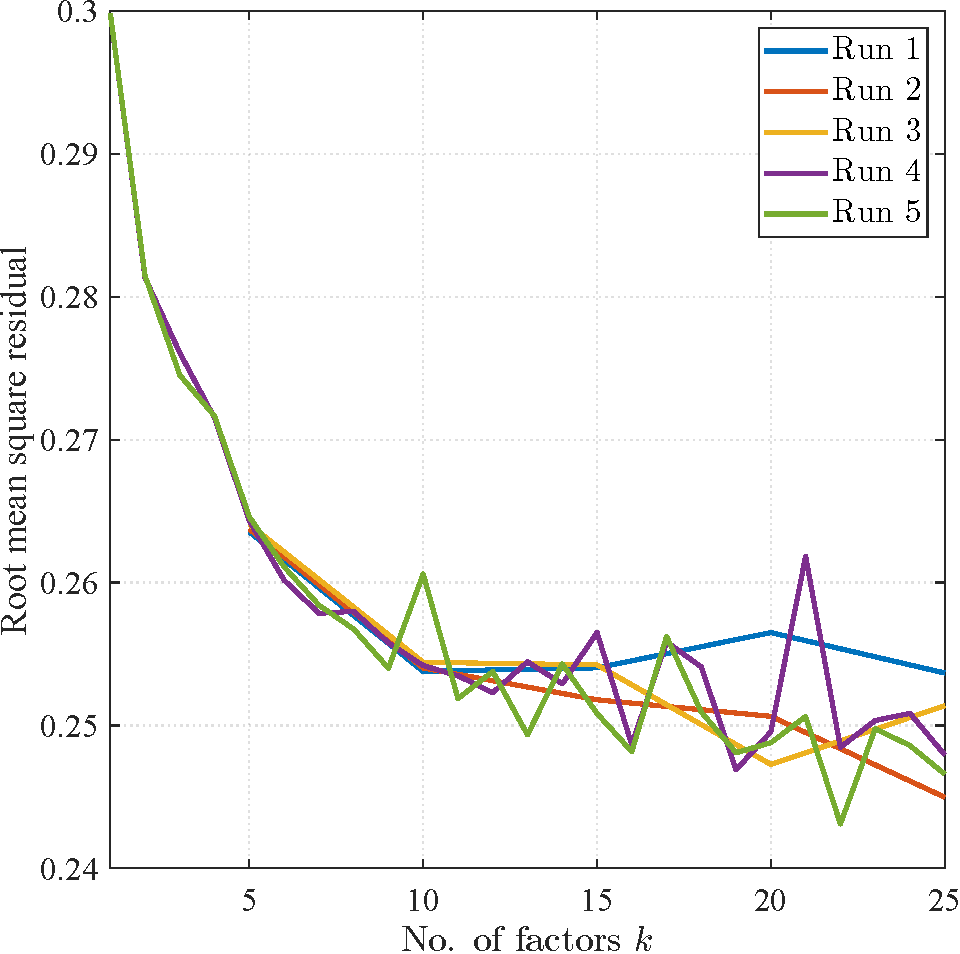
\includegraphics[width=0.99\columnwidth]{nnmf_elbow.pdf}
%		\hspace*{\fill}
%	\end{center}
%	\caption{\label{fig:nnmf_elbow} Elbow method to determine the number of factors for \ac{nnmf}.}
%\end{figure}
% ---

% Subsection ==================================================================
\subsection{Data collection}
% ---
\begin{figure}[t!]
	\begin{center}
		\hspace*{\fill}
		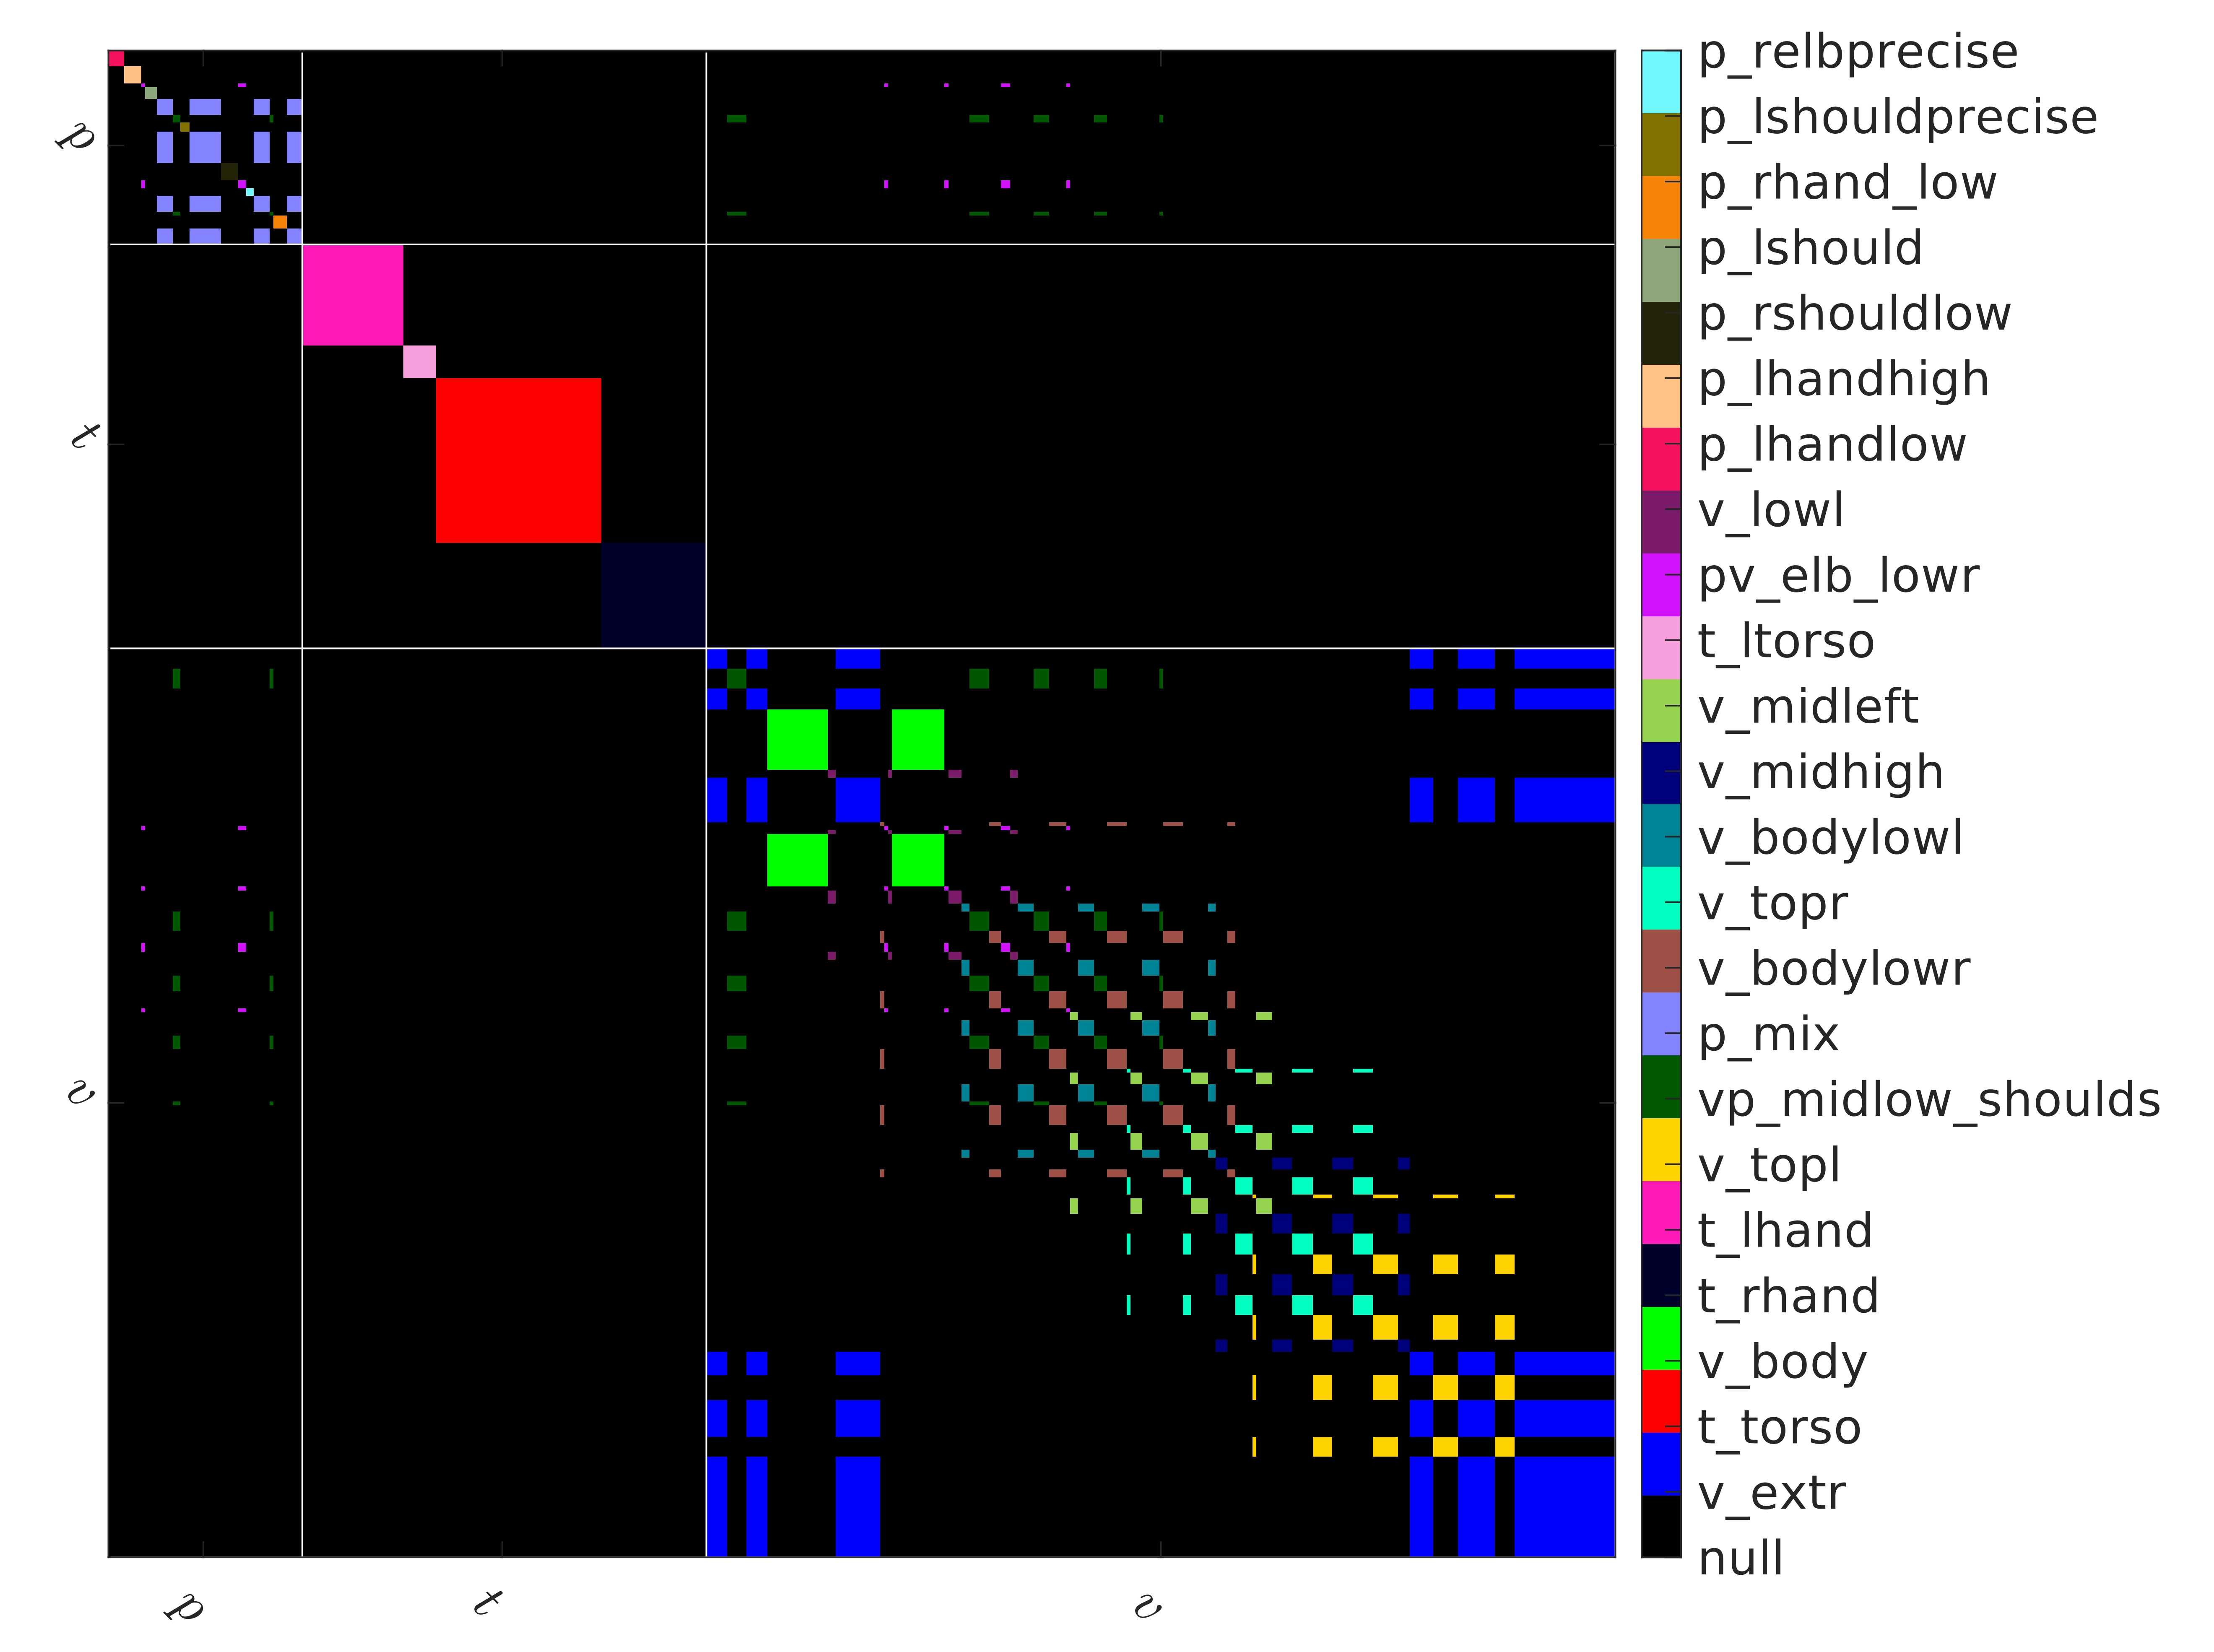
\includegraphics[width=0.9\columnwidth]{fig/irm_sensorimotor_modules.png}
		\hspace*{\fill}
	\end{center}
	\caption{\label{fig:Zmodules}. \textbf{Extracted modules from \ac{irm}.} Yellow-colored entries represent the sensors that corresponds to each extracted module (rows). From left to right, the sensory inputs are proprioceptive, tactile and visual.}
\end{figure}
% ---
The agent described in Sec.~\ref{sec:the_embidied_agent} was simulated in MATLAB for a totoal time of 30 seconds with a sampling time of 1 ms. In our experiment, we used a simple motor babbling strategy to stimulate the perceptual system and detect sensorimotpor relationships via \ac{mi}. Each antagonistic pair received a periodic muscle activation command
% --- 
\begin{equation}\label{eq:motor_babbling_torques}
	\sigma(t) =  \text{tanh} \left( A_1 \text{sin}\left(\omega_0 t\right) + A_2 \text{sin}\left(2\omega_0 t\right) + A_3 \text{sin}\left(4\omega_0 t\right) \right);
\end{equation}	
% ---
with $A_i \sim \mathcal{U}(-1,1)$, the base frequency $\omega_0 = 2\pi/T_0$, and $T_0=2$ seconds.

To compute the \ac{imi}, we used sensor signals sampled at 100 Hz and a sliding window of $T = 0.1$ seconds, i.e., the previously seen 10 samples. This short memory was stored in buffer. The selection of a relatively short time window is motivated by the fact that tactile events often occur within a short timescale. For the practical computation of the \ac{mi}
we use the open-source MATLAB package \emph{Mutual information computation} \cite{PengMutualInformationcomputation}.


% Subsection ==================================================================
\subsection{Sensorimotor modules}
The output of the IRM are modules, corresponding to a group of sensors that  have been regrouped by the IRM.


% ---
\begin{figure*}[t!]
	\begin{center}
		\hspace*{\fill}
		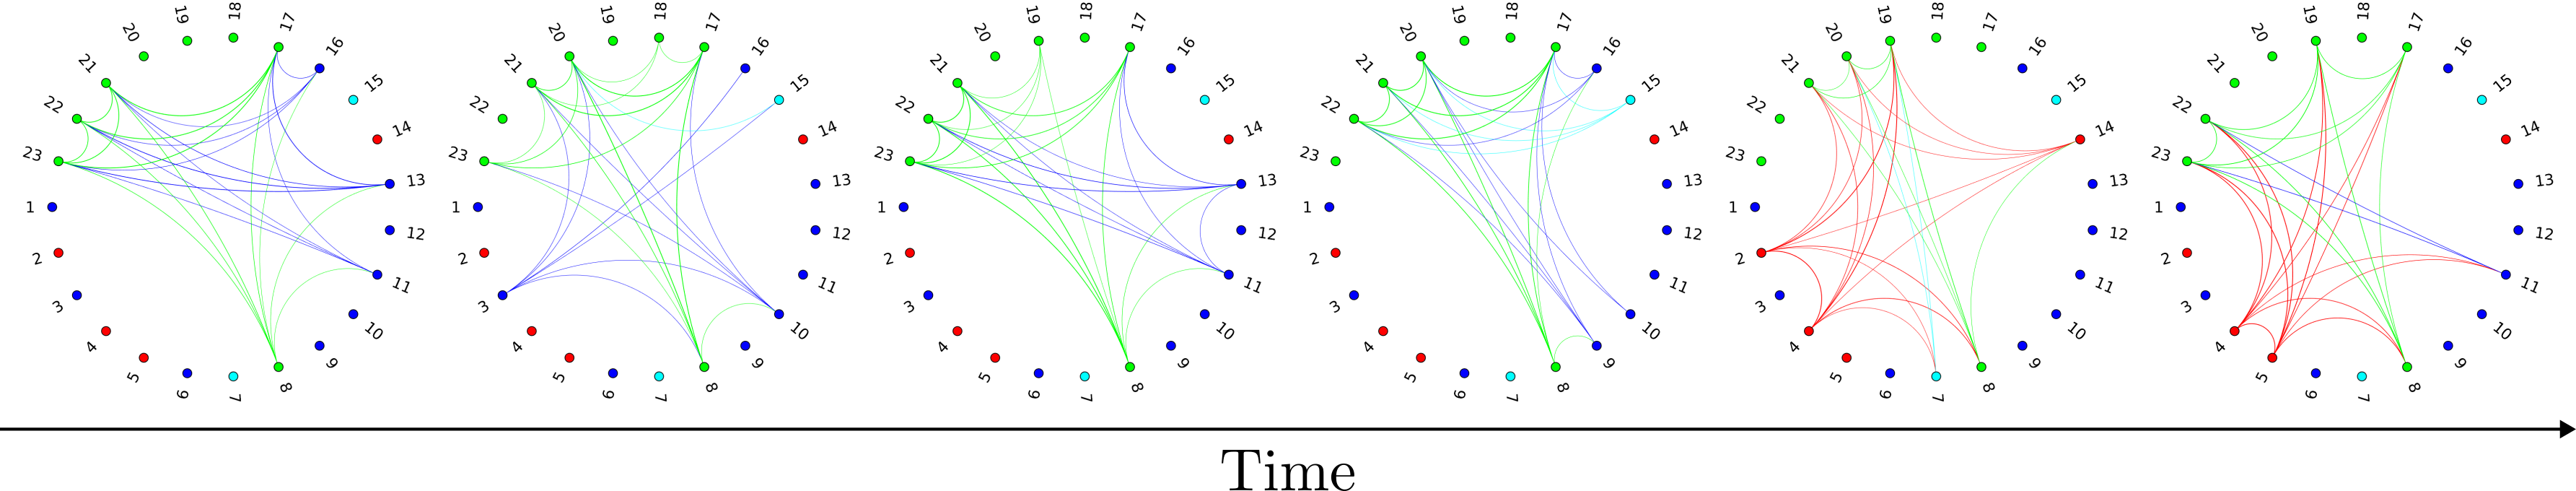
\includegraphics[width=0.9\textwidth]{fig/example_dfc.png}
		\hspace*{\fill}
	\end{center}
	\caption{\textbf{\Acl{dfc} from the \ac{irm}.} Exercpt from the time evolutoin of the connectivity between the modules found by the \acl{irm}.}
\end{figure*}
% ---

\subsection{Factors NMMF}
% ---
\begin{figure*}[!h]
	\begin{center}
		\hspace*{\fill}
		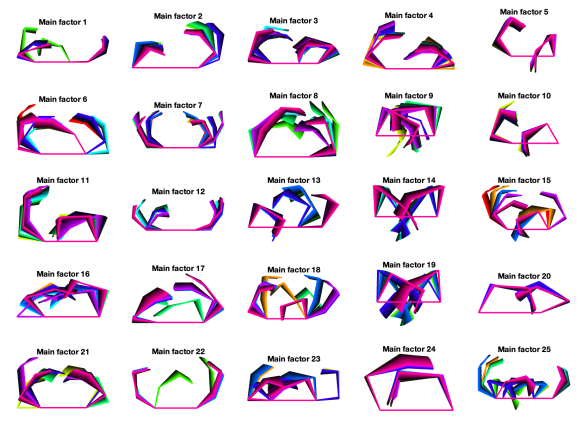
\includegraphics[width=0.99\textwidth]{fig/movement_main_factors.png}
		\hspace*{\fill}
	\end{center}
	\caption{\textbf{The factors and associated behaviors.} Different events during exploration link to a given factor; for example, pure proprioception (no touch), contact with left arm, right arm, and both arms.}
\end{figure*}
%---
\subsection{Tactile representation of Scores}
% ---
\begin{figure}[!h]
	\begin{center}
		\hspace*{\fill}
		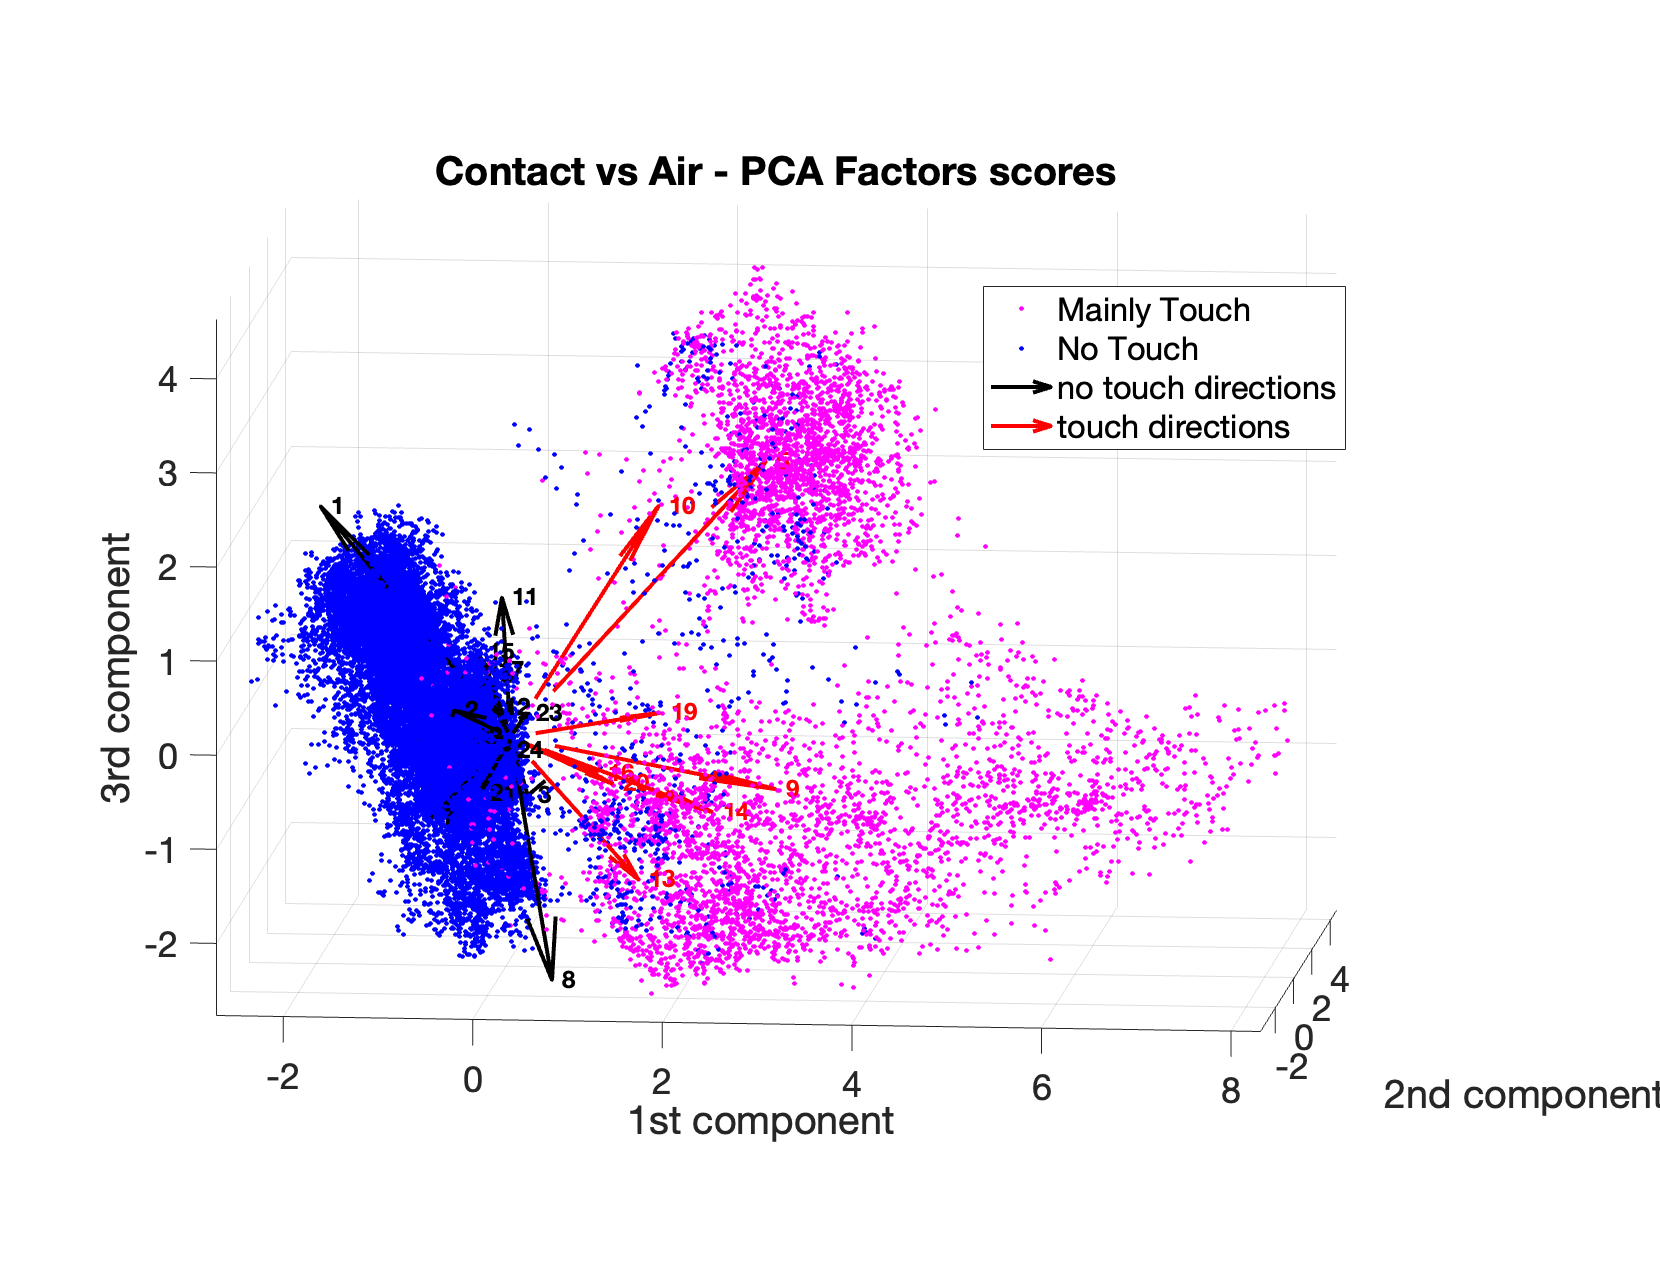
\includegraphics[width=0.99\columnwidth]{fig/pca_touch_notouch_3d.png}
		\hspace*{\fill}
	\end{center}
	\caption{\label{fig:pca3d} .}
\end{figure}
% =============================================================================
%                                                                             |
%                                                                             |

% =============================================================================
%                                                                             |
%                                                                             |
% ------------------------------- SECTION ------------------------------------|
%                                                                             |
%                                                                             |
% =============================================================================
\section{Beyond robotics}
\TODO
\pending{Valentin + Matej}

% =============================================================================
%                                                                             |
%                                                                             |
% ------------------------------- SECTION ------------------------------------|
%                                                                             |
%                                                                             |
% =============================================================================
\section{Conclusions}\label{sec:conclusion}


\section{Discussion and Future Work}

\subsection{Limitations}
One aspect not addressed is improving the motion policy used to collect the sensorimotor signals. The current study used motor babbling. However, better, perhaps goal-directed, or active exploration alternatives might lead to better results that are able to capture and reproduce particular sensorimotor behaviors.

The current implementation of our framework requires collecting and processing information offline. A method capable of doing online learning with the potential to adapt, for example, the clusters or the factors, is still an open question.

It is possible to add factors.

\printbibliography 
\end{document}